\documentclass[aspectratio=169,11pt,hyperref={colorlinks=true}]{beamer}
\usetheme{boxes}
\setbeamertemplate{navigation symbols}{}
\definecolor{ibm}{RGB}{70,107,176}
\setbeamercolor{titlelike}{fg=ibm}
\setbeamercolor{structure}{fg=ibm}
\hypersetup{colorlinks,urlcolor=ibm}
\setbeamertemplate{footline}[frame number]
% Inserting graphics
\usepackage{graphicx}
% Side-by-side figures, etc
\usepackage{subfigure}
% Code snippits
%\usepackage{listings}
\usepackage{minted}

\usepackage{lmodern}
% Color stuff
\usepackage{color}
\usepackage{amsmath}
\usepackage{amssymb}
\usepackage{empheq}
\usepackage{gensymb}
\newcommand\RBox[1]{%
  \tikz\node[draw,rounded corners,align=center,] {#1};%
}
\usepackage{hyperref}
\usepackage[T1]{fontenc}

\definecolor{mygreen}{rgb}{0,0.6,0}
\definecolor{mygray}{rgb}{0.5,0.5,0.5}
\definecolor{mymauve}{rgb}{0.58,0,0.82}

\setbeamerfont{caption}{series=\normalfont,size=\fontsize{6}{8}}
\setbeamertemplate{caption}{\raggedright\insertcaption\par}

\setlength{\abovecaptionskip}{0pt}
\setlength{\floatsep}{0pt}

\author[Matthew Treinish]{%
    \texorpdfstring{%
        \centering
        Matthew Treinish\\
        Senior Software Engineer - IBM Research\\
        \href{mailto:mtreinish@kortar.org}{mtreinish@kortar.org}\\
        \href{https://github.com/mtreinish/rustwork-presentation}{https://github.com/mtreinish/rustwork-presentation}
   }
   {Matthew Treinish}
}
\date{June 18, 2024}

\title{Rustworkx}
\begin{document}

\titlepage
\section{Rustworkx Introduction}
\begin{frame}
    \frametitle{What is Rustworkx?}
    \begin{columns}
        \column{.5\textwidth}
            \begin{itemize}
                \item Open source graph library written in Rust
                \item Primarily a library for Python
                \item Designed for high performance and flexibility
                \item Apache 2.0 Licensed
            \end{itemize}
        \column{.5\textwidth}
            \centering
            
\includegraphics[width=.8\textwidth]{rustworkx_logo.png}\\
            \footnotesize
            \textit{Unofficial logo, see}:\\ \href{https://github.com/Qiskit/rustworkx/issues/824}{https://github.com/Qiskit/rustworkx/issues/824}
    \end{columns}
\end{frame}

\begin{frame}
    \frametitle{Origin of the project}
    \begin{columns}
        \column{.5\textwidth}
        \begin{itemize}
            \item Started as a library to replace NetworkX usage for the Qiskit\footnotemark compiler's DAG IR.
            \item Use case where a graph is built, analyzed, mutated, and analyzed again as part of compiler transforms.
            \item Designed to be flexible so that any Python object can be attached to a graph
            \item Expanded to cover other graph functionality
        \end{itemize}
        \column{.5\textwidth}
        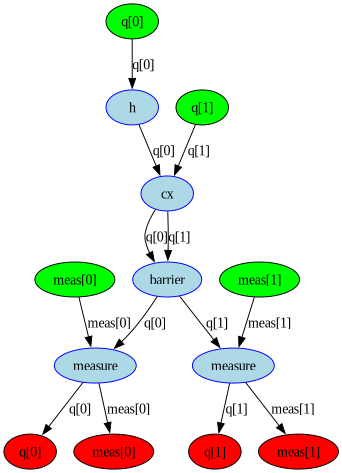
\includegraphics[height=.8\textheight]{dag.png}
    \end{columns}
    \footnotetext[1]{Javadi-Abhari, A., Treinish, M., Krsulich, K., Wood, C. J., Lishman, J., Gacon, J., \ldots \& Gambetta, J. M. (2024). Quantum computing with Qiskit. arXiv preprint arXiv:2405.08810. \href{ihttps://doi.org/10.48550/arXiv.2405.08810}{https://doi.org/10.48550/arXiv.2405.08810}}
\end{frame}

\begin{frame}
    \frametitle{Why Rust?}
    \begin{columns}
        \column{.5\textwidth}
            \begin{itemize}
                \item Rust is designed for safety with no runtime
                \item Compiler checks to make sure it's memory safe and has safe concurrency
                \item Performance of Rust code is equivalent to C or C++ but has the safety guarantees
                \item Rust packaging and build tooling make integration with Python simple
            \end{itemize}
        \column{.5\textwidth}
            
\includegraphics[width=\textwidth]{rust-logo-512x512.png}
    \end{columns}
    \footnotetext[1]{Matsakis, N. D., \& Klock, F. S. (2014). The rust language. ACM SIGAda Ada Letters, 34(3), 103-104. \href{https://doi.org/10.1145/2692956.2663188}{https://doi.org/10.1145/2692956.2663188}}
\end{frame}

\subsection{Using Rustworkx}
\begin{frame}
    \frametitle{Two Language Bindings}
    \begin{columns}
        \column{.5\textwidth}
        \textbf{Python Library}
        \begin{itemize}
            \item Primary Interface
            \item Python library for creating graphs
            \item Enables using any Python object for node and edge payloads
            \item Visualization functions for using \href{https://matplotlib.org/}{Matplotlib} and \href{https://graphviz.org/}{Graphivz}
            \item Package available on \href{https://pypi.org/project/rustworkx/}{PyPI} for Linux (x86\_64, i686, ppc64le, s390x, aarch64), Windows (32bit and 64bit), MacOS (x86\_64, arm64).
        \end{itemize}
        \column{.5\textwidth}
        \textbf{Rust Library}
        \begin{itemize}
            \item Rust language library that provides rust implementation of graph algorithms
            \item Currently built as an extension to \href{https://docs.rs/petgraph/latest/petgraph/}{petgraph} library
            \item Pure rust library (no Python needed)
            \item Designed to be generic to work with with arbitrary data types
            \item Used to build the Python library
        \end{itemize}
    \end{columns}
\end{frame}

\begin{frame}
    \frametitle{Rust interface}
    \inputminted{Rust}{rust_example.rs}
\end{frame}

\begin{frame}
    \frametitle{Python Interface}
    \inputminted{Python}{python_example.py}
\end{frame}

\begin{frame}
    \frametitle{Using Rustworkx}
    \begin{columns}
        \column{.5\textwidth}
            \begin{itemize}
            \only<1->{\item Two classes PyGraph and PyDiGraph for undirected and directed graphs respectively}
            \only<2->{\item All nodes and edges are addressed with integer indices and data payloads can be any Python object}
            \only<3->{\item Graphs can be multigraphs (the default)}
            \only<4>{\item Callbacks are typically used to convert data payloads to static types for algorithms}
            \end{itemize}
        \column{.5\textwidth}
            \only<1>{\scriptsize \inputminted{python}{graph_classes.py}}
            \only<2>{\scriptsize \inputminted{python}{index.py}}
            \only<3>{\scriptsize \inputminted{python}{multigraph.py}}
            \only<4>{\scriptsize \inputminted{python}{callbacks.py}}
    \end{columns}
\end{frame}

\section{Benchmarks}
\begin{frame}
    \frametitle{Benchmarks with Random Barabási-Albert graphs\footnotemark}
    \begin{columns}
        \column{.5\textwidth}
            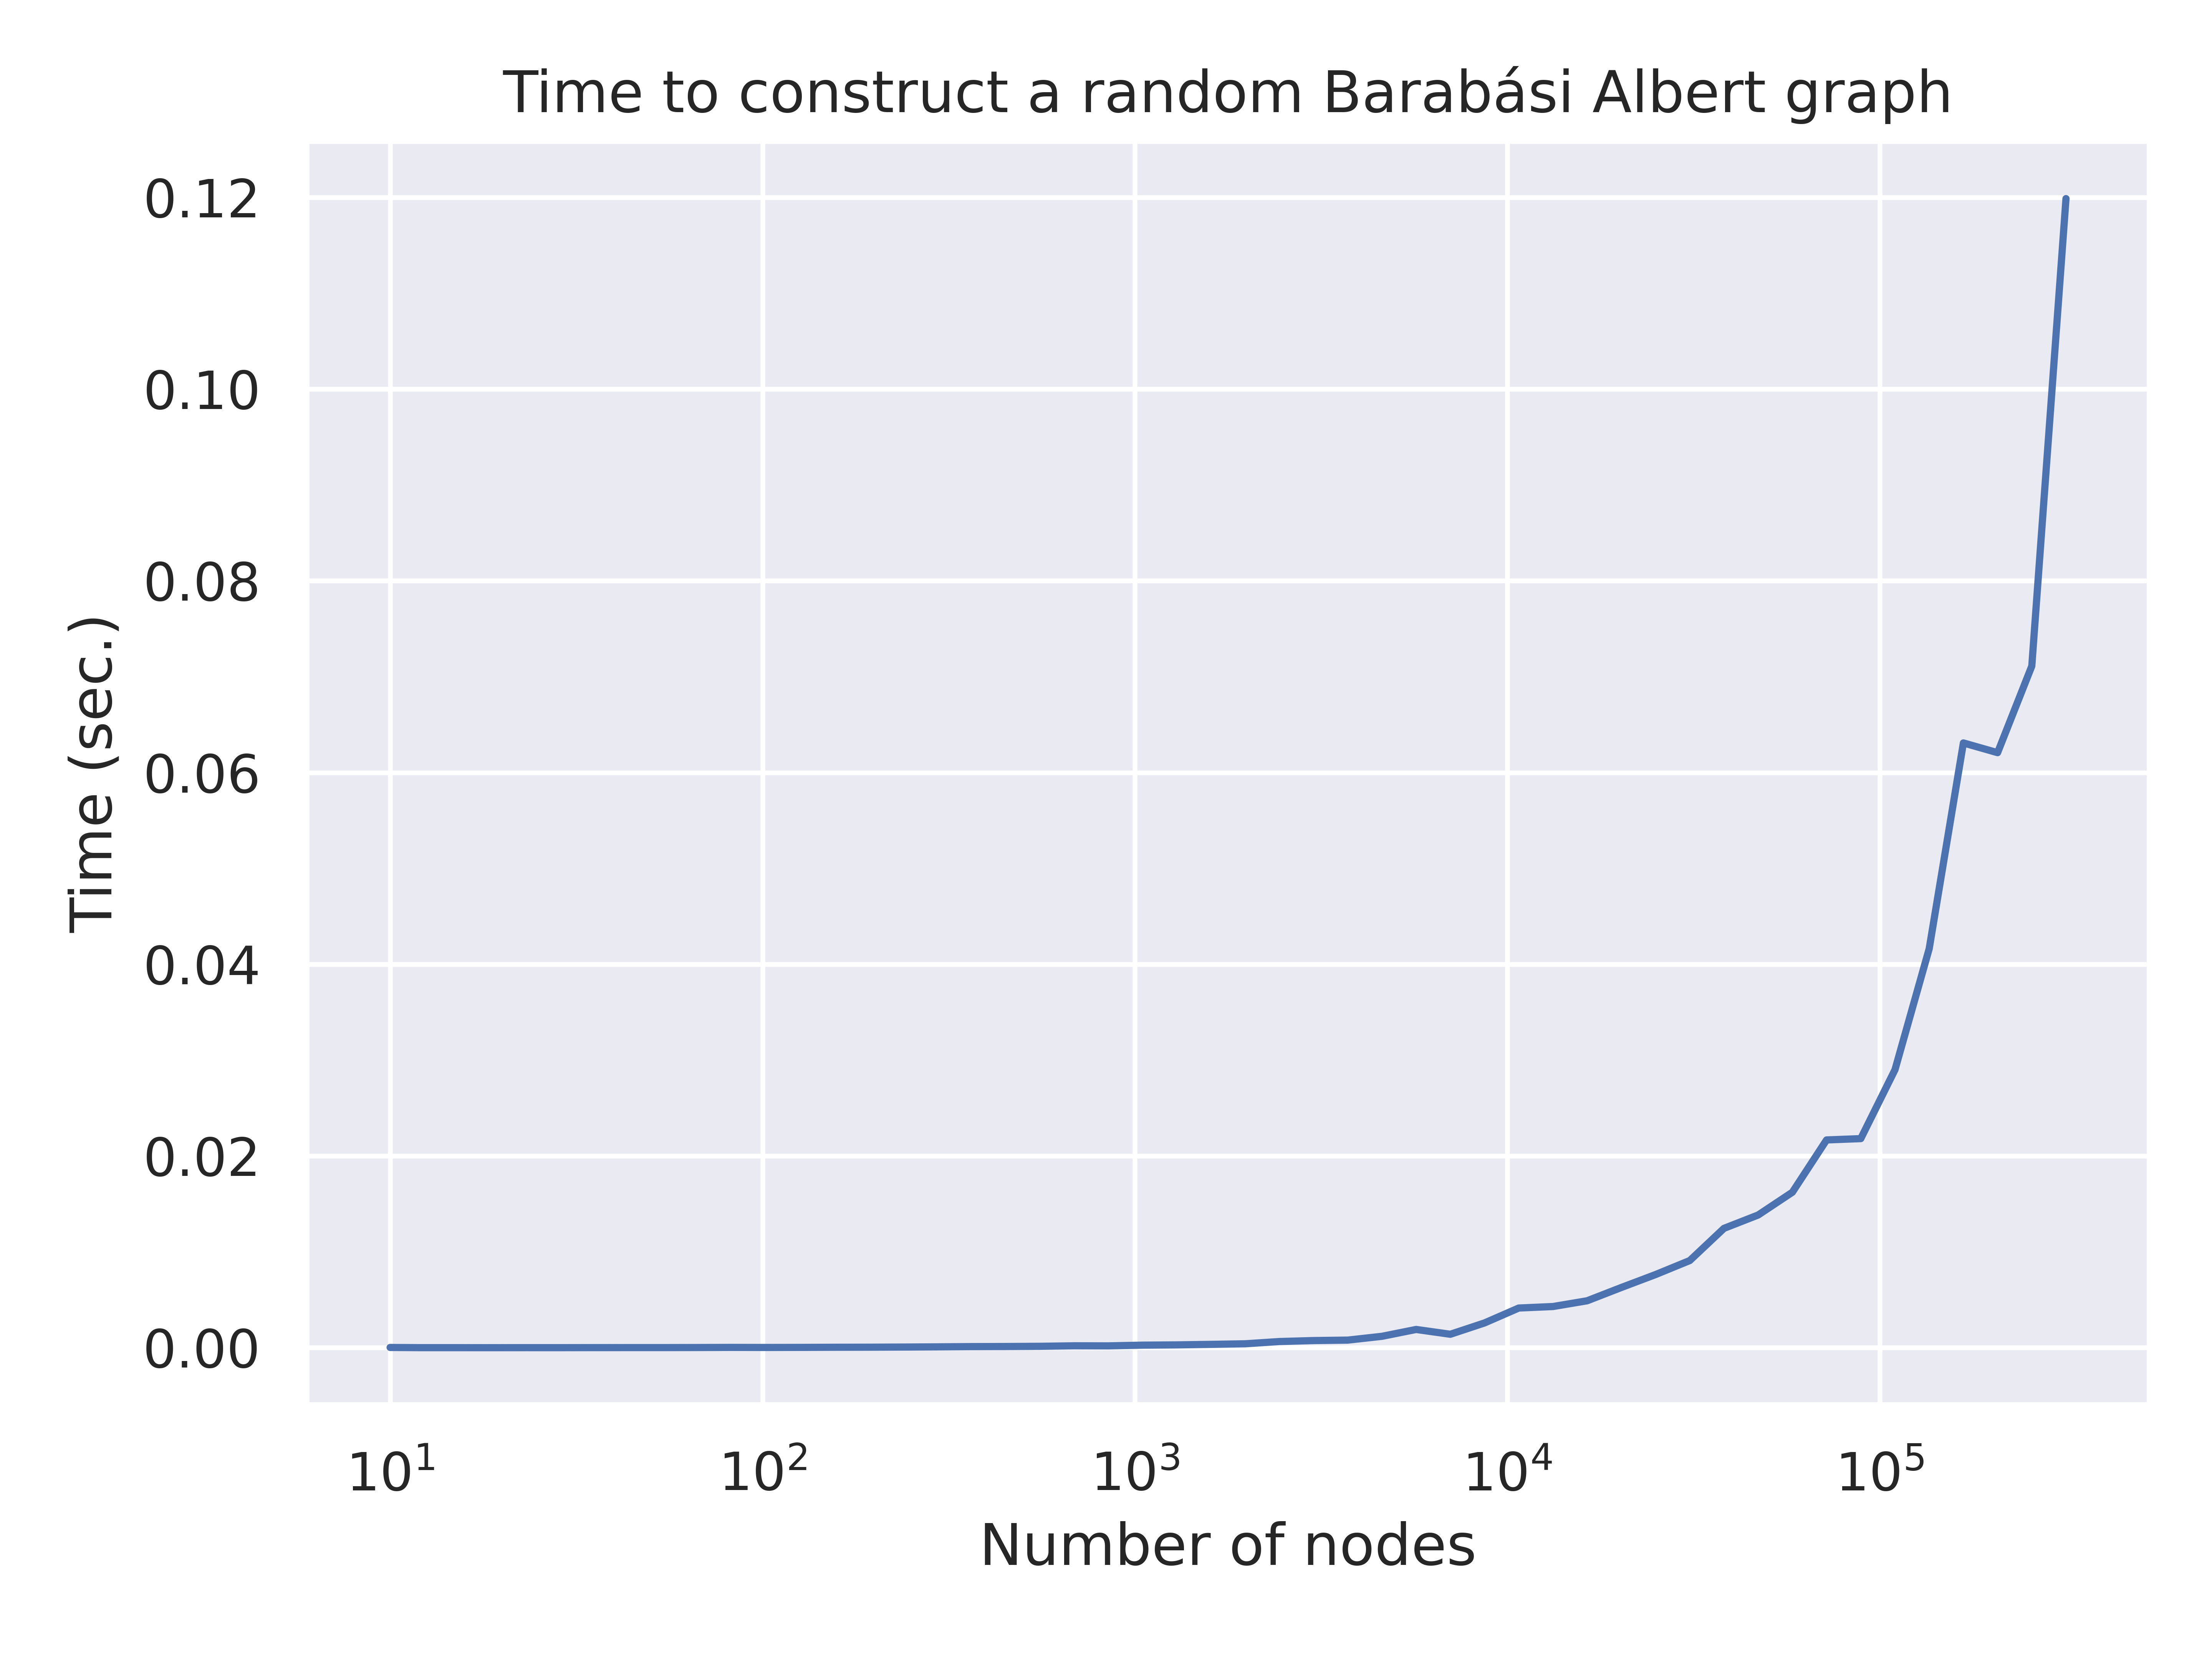
\includegraphics[width=\textwidth]{albert-graph_time.png} \\
        \column{.5\textwidth}
            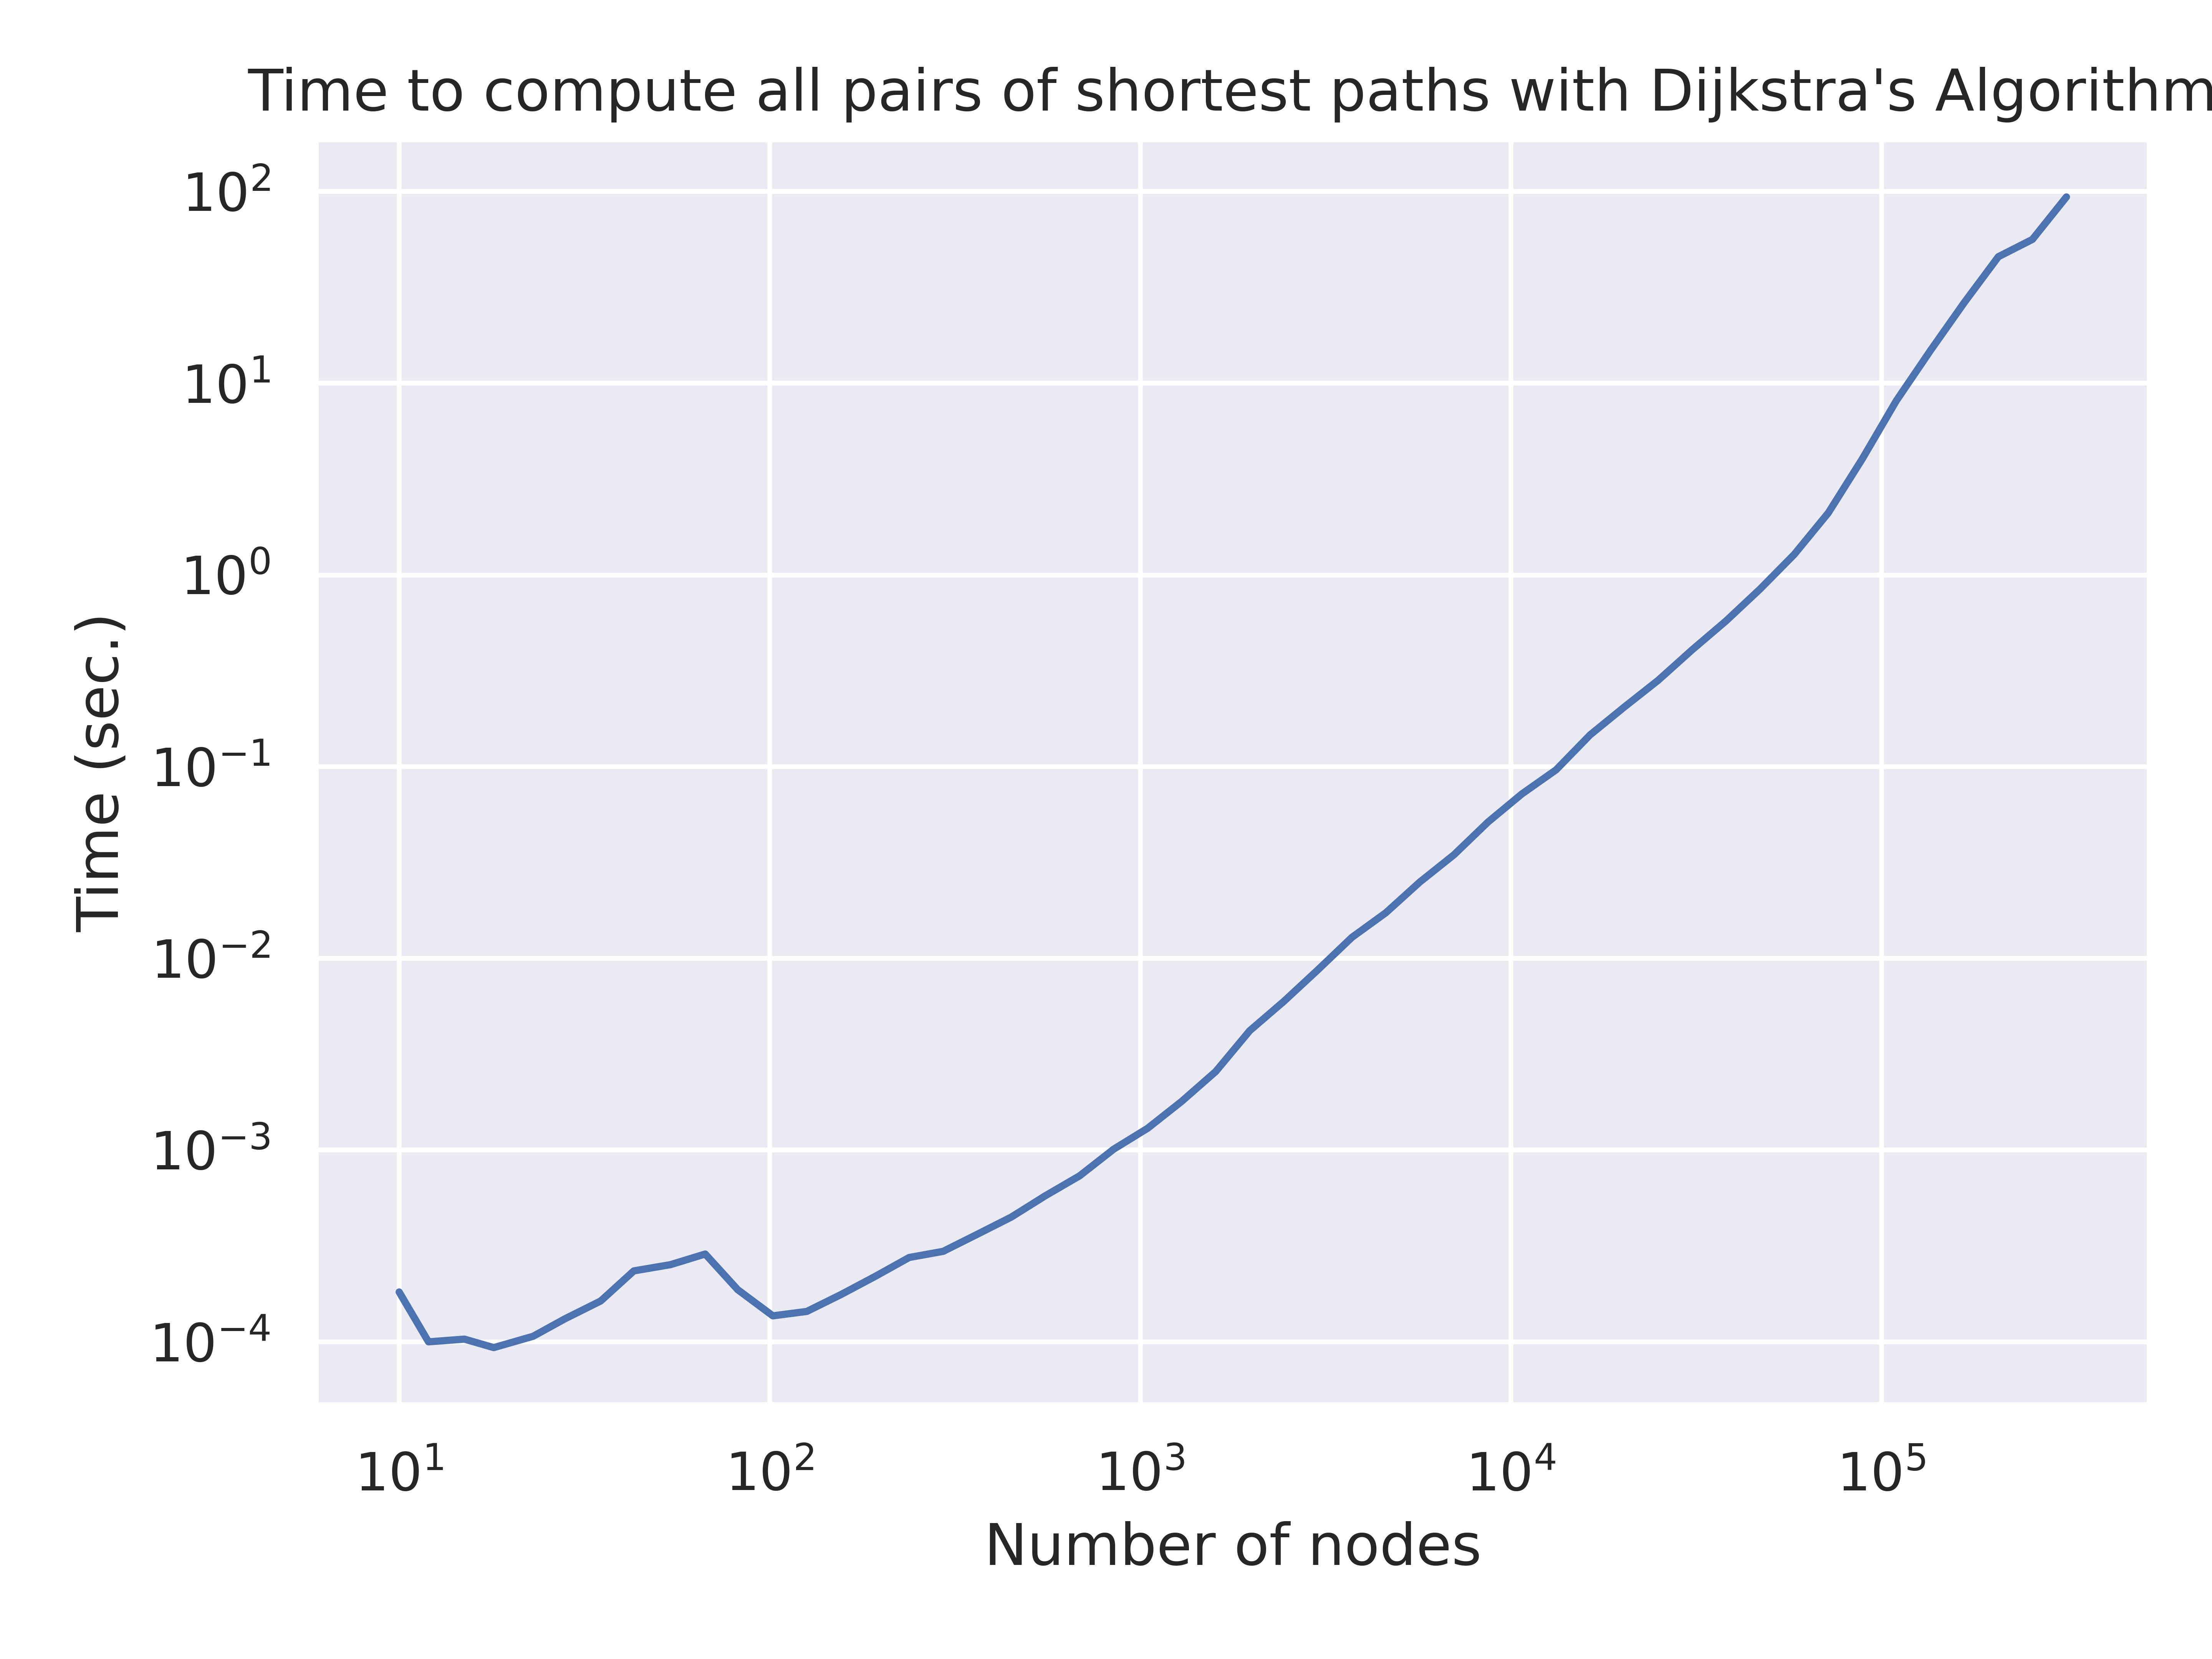
\includegraphics[height=.45\textheight]{shortest_path.png} \\
            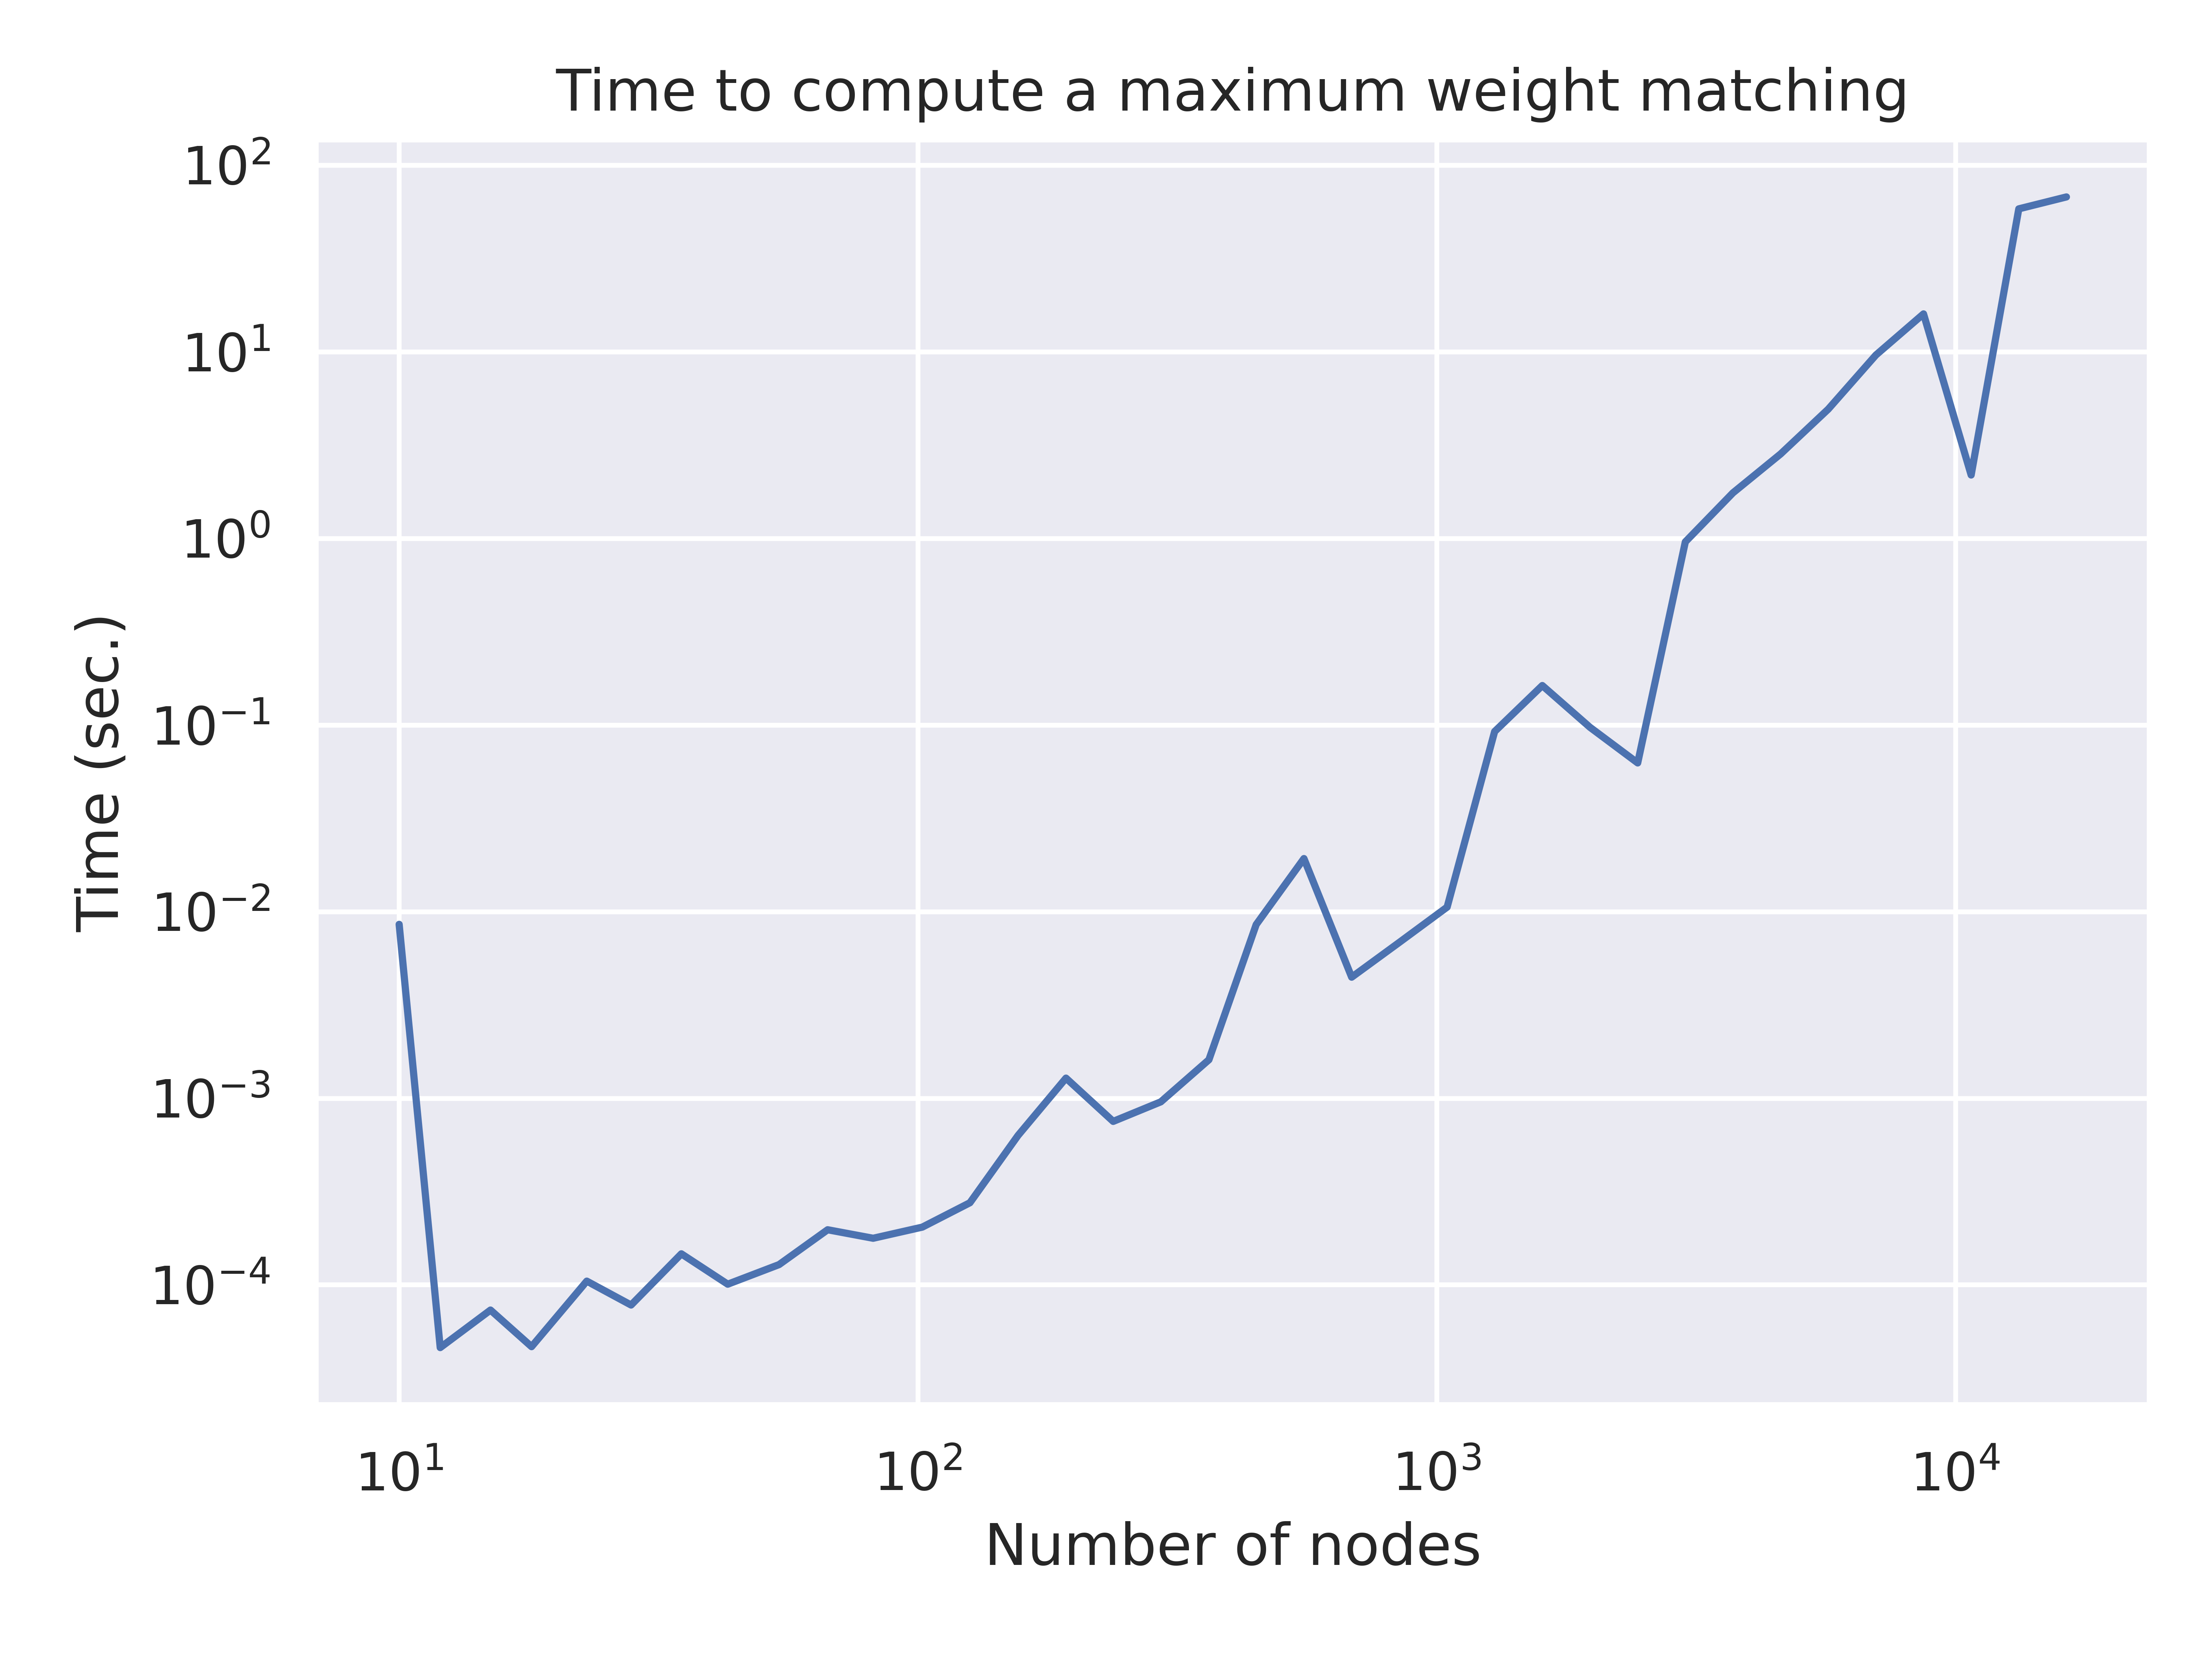
\includegraphics[height=.45\textheight]{max_weight.png} \\
    \end{columns}
    \footnotetext[2]{Barabási, A. L., \& Albert, R. (1999). Emergence of scaling in random networks. science, 286(5439), 509-512. \href{https://doi.org/10.1126/science.286.5439.509}{https://doi.org/10.1126/science.286.5439.509}}
\end{frame}

\begin{frame}
    \frametitle{All Pairs shortest path for Road Network of Rome, Italy in 1999\footnotemark}
    \centering
    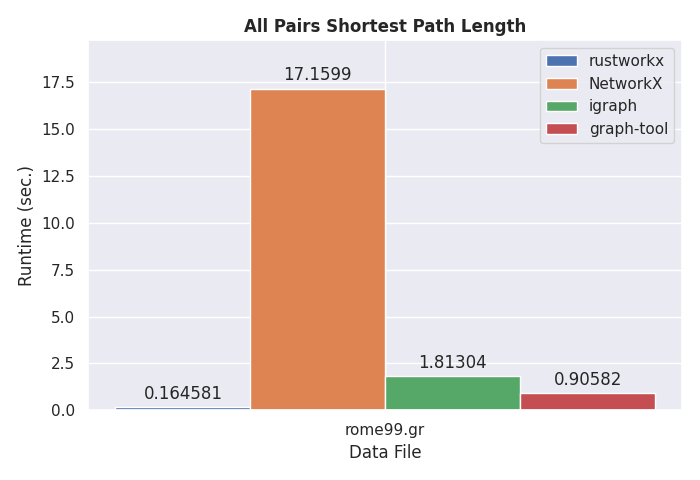
\includegraphics[height=.8\textheight]{all_pairs.png}
    \footnotetext[3]{Demetrescu, C., Goldberg, A., \& Johnson, D. The Shortest Path Problem: Ninth DIMACS Implementation Challenge. \href{https://doi.org/10.1090/dimacs/074}{https://doi.org/10.1090/dimacs/074}}
\end{frame}

\begin{frame}
    \frametitle{Subgraph isomorphism benchmarks using ARG database\footnotemark}
    \centering
    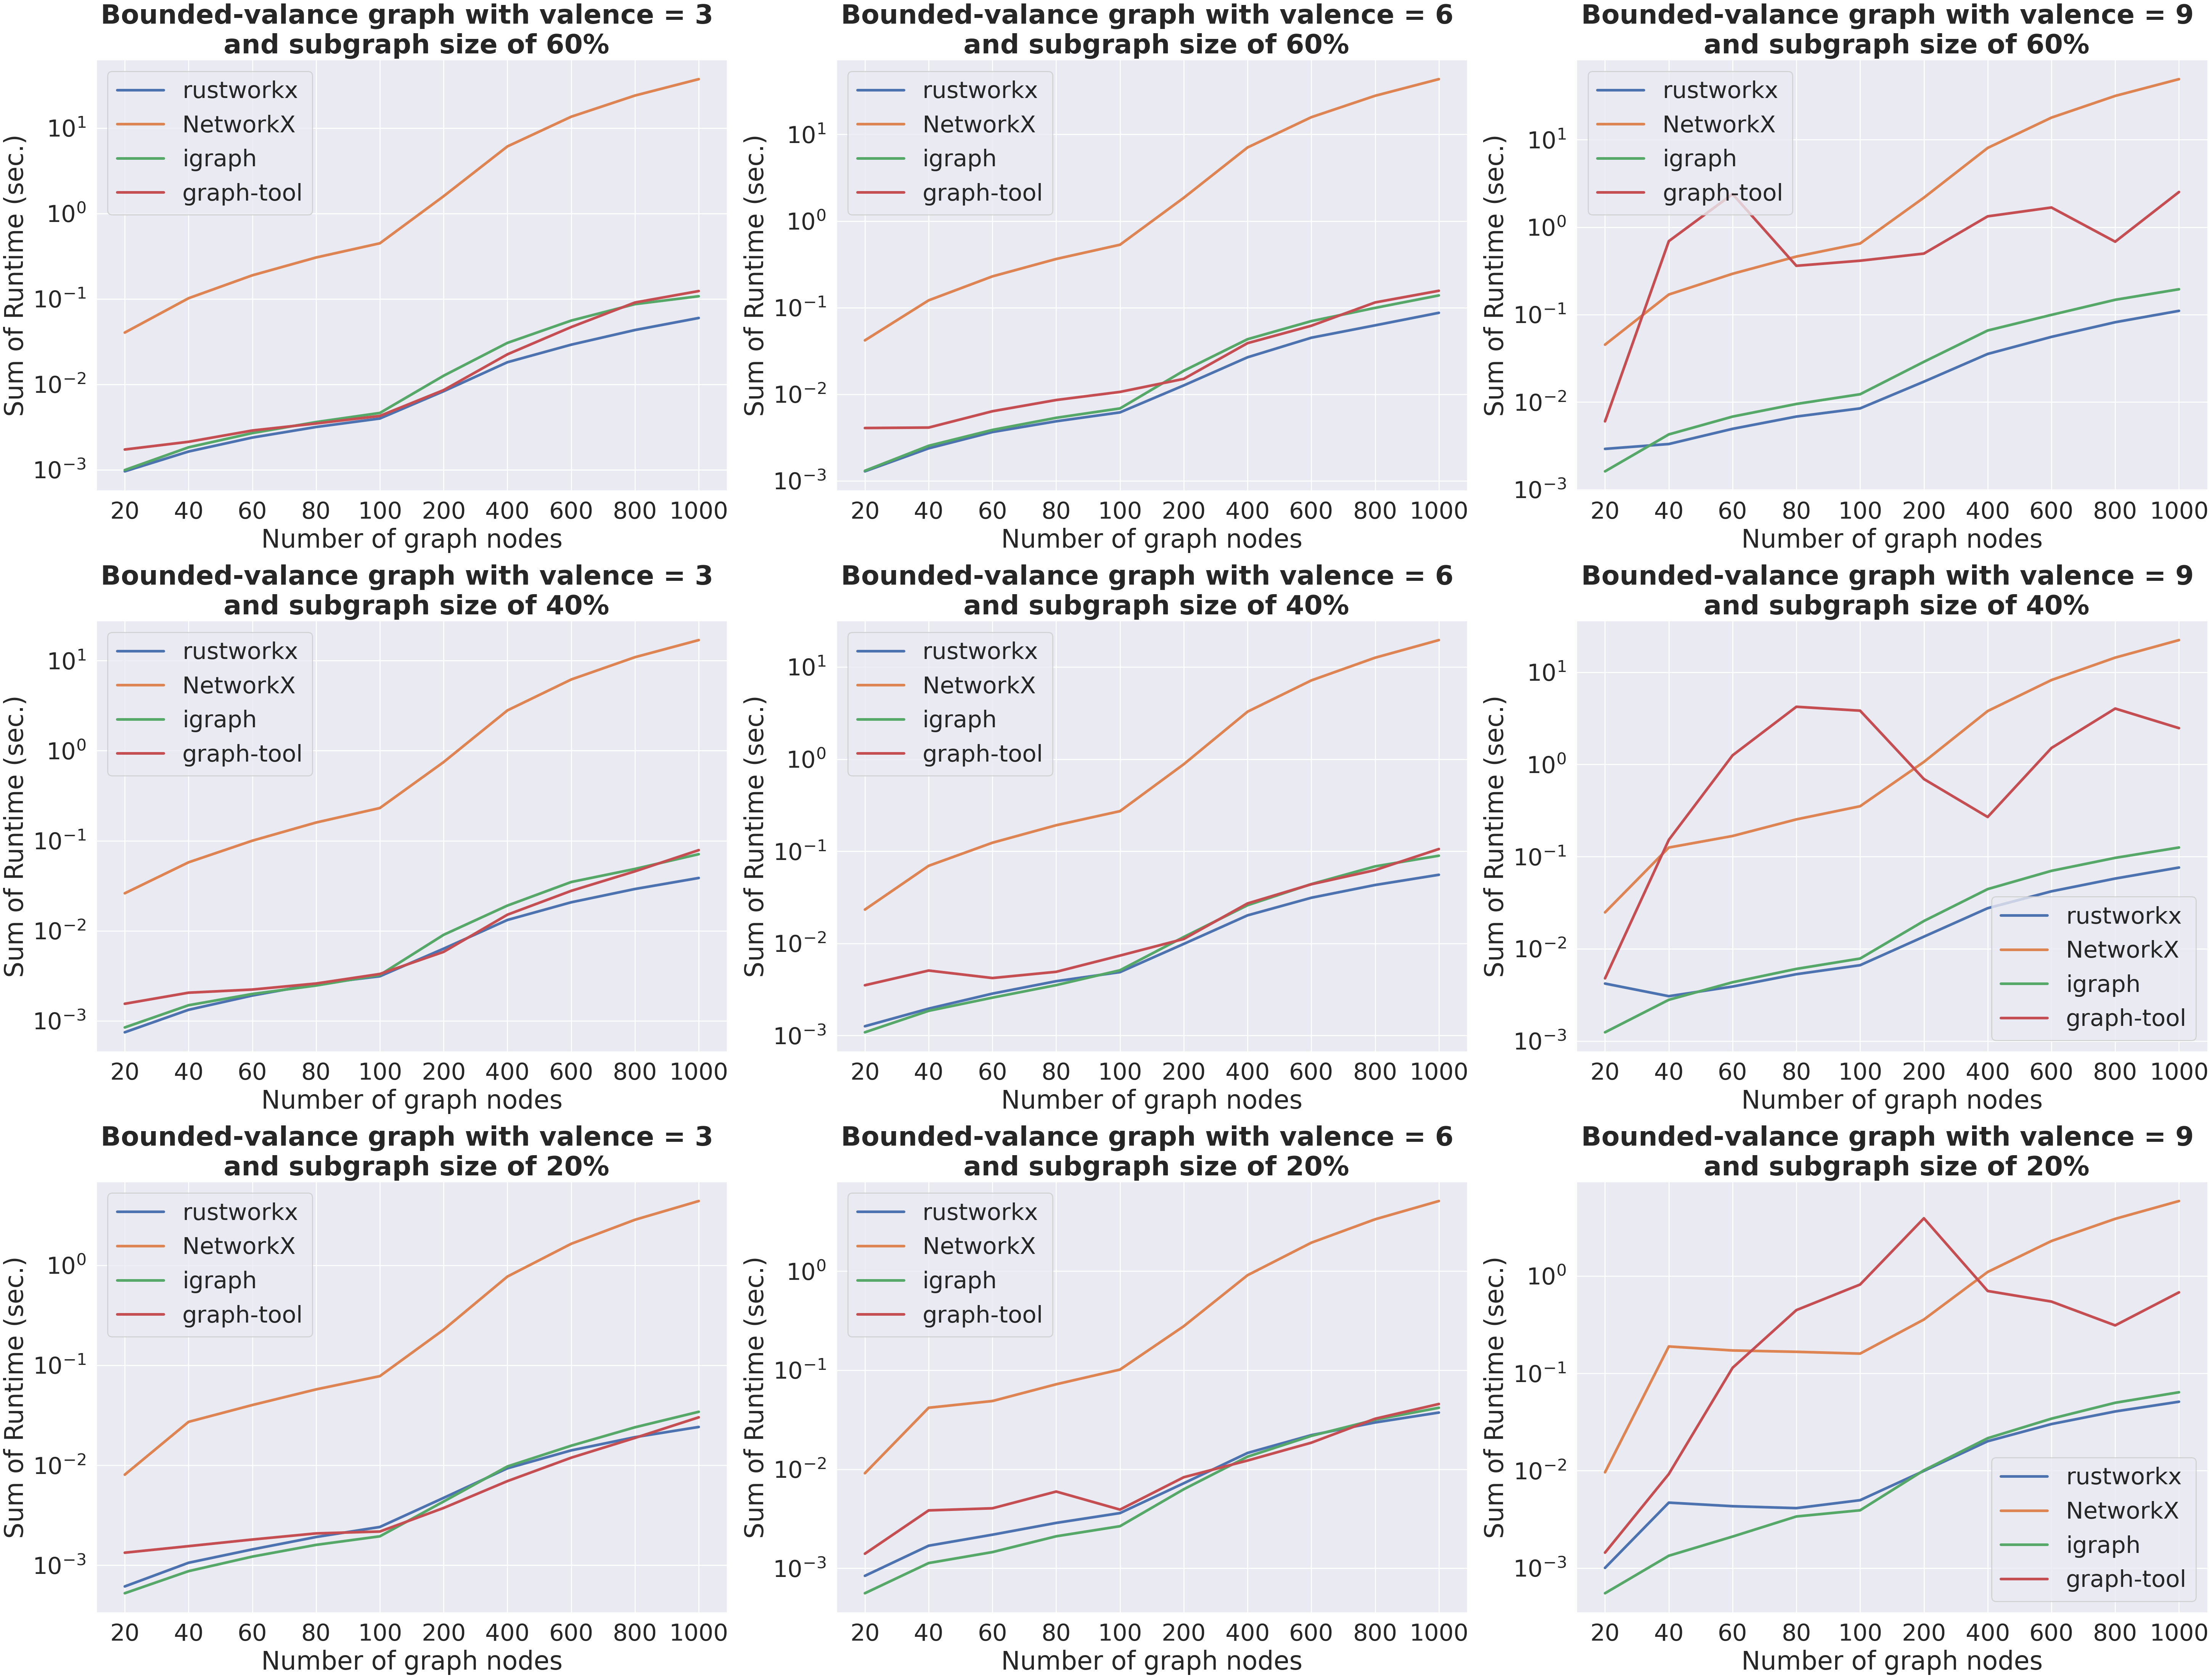
\includegraphics[height=.75\textheight]{subgraph_isomorphism.png}
    \footnotetext[4]{Santo, M. D., Foggia, P., Sansone, C., \& Vento, M. (2003). A large database of graphs and its use for benchmarking graph isomorphism algorithms. Pattern Recognition Letters, 24(8), 1067–1079. \href{https://doi.org/10.1016/S0167-8655(02)00253-2}{https://doi.org/10.1016/S0167-8655(02)00253-2}}
\end{frame}

\section{Examples using rustworkx}
\begin{frame}
    \frametitle{Subgraph Isomorphism based Quantum Circuit Layout\footnotemark}
    \only<1> {\centering 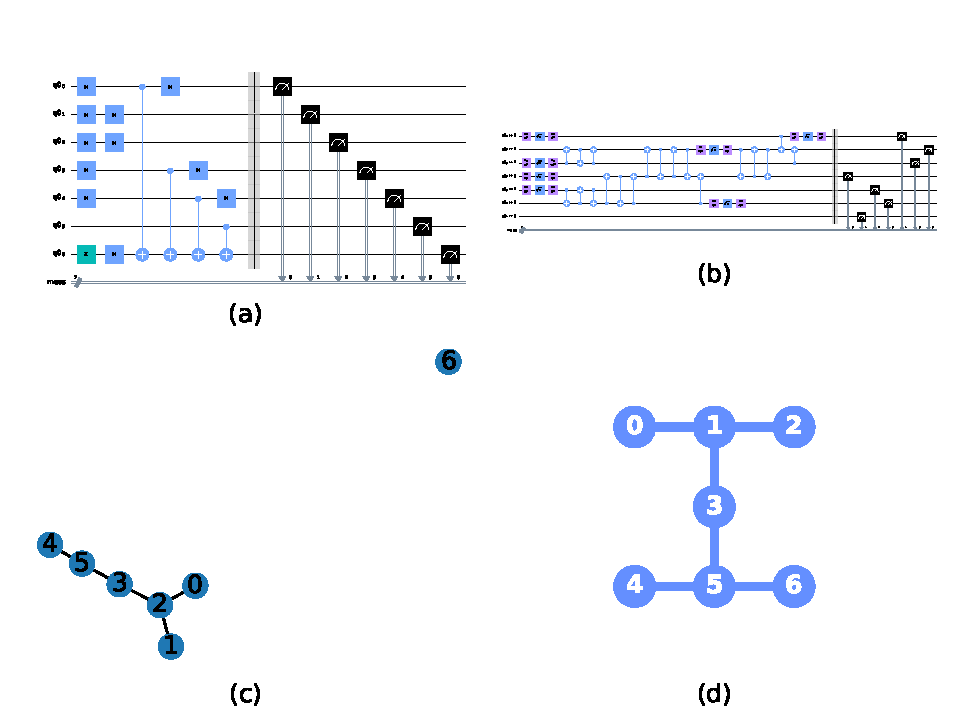
\includegraphics[height=.8\textheight]{vf2_overview.pdf}}
    \only<2> {\scriptsize \inputminted{Python}{vf2_layout_build.py}}
    \only<3> {\scriptsize \inputminted{Python}{vf2_layout_map.py} 
    \tiny
    Find best subgraph using VF2 with ordering heuristic from VF2++\footnotemark}

    \footnotetext[5]{Nation, P. D., \& Treinish, M. (2023). Suppressing quantum circuit errors due to system variability. PRX Quantum, 4(1), 010327. \href{https://doi.org/10.1103/PRXQuantum.4.010327}{https://doi.org/10.1103/PRXQuantum.4.010327}}
    \only<3> {\footnotetext[6]{Jüttner, A., \& Madarasi, P. (2018). VF2++—An improved subgraph isomorphism algorithm. Discrete Applied Mathematics, 242, 69-81. \href{https://doi.org/10.1016/j.dam.2018.02.018}{https://doi.org/10.1016/j.dam.2018.02.018}}}
\end{frame}

\begin{frame}
    \frametitle{Uses Outside of Quantum Computing}
    \footnotesize
    \begin{itemize}
        \item Rautila, O. S., Kaivola, K., Rautila, H., Hokkanen, L., Launes, J., Strandberg, T. E., \ldots \& Tienari, P. J. (2024). The shared ancestry between the C9orf72 hexanucleotide repeat expansion and intermediate-length alleles using haplotype sharing trees and HAPTK. The American Journal of Human Genetics, 111(2), 383-392. \href{https://doi.org/10.1016/j.ajhg.2023.12.019}{https://doi.org/10.1016/j.ajhg.2023.12.019}
        \item Chen, R., Ding, Z., Zheng, S., Zhang, C., Leng, J., Liu, X., \& Liang, Y. (2024, April). Magis: Memory optimization via coordinated graph transformation and scheduling for dnn. In Proceedings of the 29th ACM International Conference on Architectural Support for Programming Languages and Operating Systems, Volume 3 (pp. 607-621). \href{https://doi.org/10.1145/3620666.3651330}{https://doi.org/10.1145/3620666.3651330}
        \item Tantos A, Kosmidis K. From Discourse Relations to Network Edges: A Network Theory Approach to Discourse Analysis. Applied Sciences. 2023; 13(12):6902. \href{https://doi.org/10.3390/app13126902}{https://doi.org/10.3390/app13126902}
        \item Caetano, J., Carriço, N., Figueira, J. R., \& Covas, D. (2023). A novel methodology for pipe grouping and rehabilitation interventions scheduling in water distribution networks. Urban Water Journal, 20(7), 769–781. \href{https://doi.org/10.1080/1573062X.2023.2209560}{https://doi.org/10.1080/1573062X.2023.2209560}
        \item Setiawan, T. H., Beltsazar, F., Aden, A., Gunawan, G., \& Zarista, R. H. (2023). Graph coloring for determining courier frequency. Desimal: Jurnal Matematika, 6(3), 273 - 284.
    \end{itemize}
\end{frame}

\section{Questions?}
\begin{frame}
\frametitle{Where to get more information}
    \begin{itemize}
        \item These Slides: \href{https://github.com/mtreinish/rustwork-presentation}{https://github.com/mtreinish/rustwork-presentation}
        \item Rustworkx Documentation: \href{https://www.rustworkx.org}{https://www.rustworkx.org}
        \item Tutorial for NetworkX users: \href{https://www.rustworkx.org/networkx.html}{https://www.rustworkx.org/networkx.html}
        \item Rustworkx on Github: \href{https://github.com/Qiskit/rustworkx}{https://github.com/Qiskit/rustworkx}
        \item JOSS Paper: \href{https://joss.theoj.org/papers/10.21105/joss.03968}{https://joss.theoj.org/papers/10.21105/joss.03968}
    \end{itemize}
\end{frame}
\end{document}
